\documentclass{beamer}

\title{Analyse des enlèvements}
\author{Fournisseur: \textbf{}}
\titlegraphic{\vspace*{0.5cm} 
\includegraphics[width=5cm]{images/leclerc}}
\date{Avril à Juin 2024}

\setlength{\parskip}{0.2cm}
\usepackage[font=tiny]{caption}

\begin{document}
    \begin{frame}
        \titlepage
    \end{frame}

    \begin{frame}
        \frametitle{Table des matières}
        \tableofcontents
    \end{frame}

    \section{Introduction}

    \begin{frame}
        \tiny
        \frametitle{Introduction}
        Ce rapport traite les données du mois de Avril à Juin 2024. Il analyse en détail les achats de nos points de vente.\par

        Quelques informations clefs :

        \begin{itemize}
            \item{Le \textbf{CA} total du mois dernier s’élève à \textbf{32 865.70€}.}
            \item{\textbf{15 030 UVC} ont été commandés le mois dernier par nos points de vente}
            \item{\textbf{47 références} articles ont été commandées}
            \item{\textbf{4 points de vente} ont commandé vos articles}
            \item{Voici la liste des points de vente qui n’ont pas réalisé de commande sur vos références le mois dernier : A, B, C.}
        \end{itemize}

        Dans la première partie, l’analyse est détaillée par point de vente.\par
        Dans la deuxième partie, l’analyse est détaillée par mode de gestion.\par
        Dans la troisième partie, l’analyse est détaillée par article.\par
        Pour rappel, vous avez souscrit au contrat Contrat ABC le 11 mars 2024 pour une mise à disposition des données mensuelles détaillées à l’article et par point de vente.\par
    \end{frame}

    \section{Analyse des points de vente}

    \begin{frame}
        \tiny
        \frametitle{Analyse des points de vente}

        Les visualisations ci-dessous représente le CA (PERMANENT + NON PERMANENT) par points de vente.\par

        
                    \begin{columns}
                                    \column{0.3333333333333333\textwidth}
                        \centering
                        \begin{figure}[h]
                            \centering
                            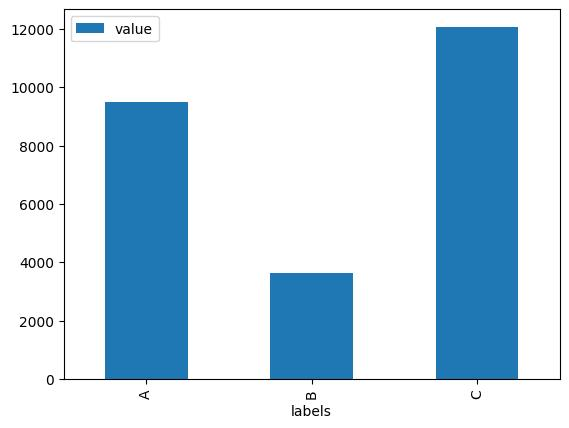
\includegraphics[width=1\textwidth]{assets/ca_0.jpg}
                        \end{figure}
                                    \column{0.3333333333333333\textwidth}
                        \centering
                        \begin{figure}[h]
                            \centering
                            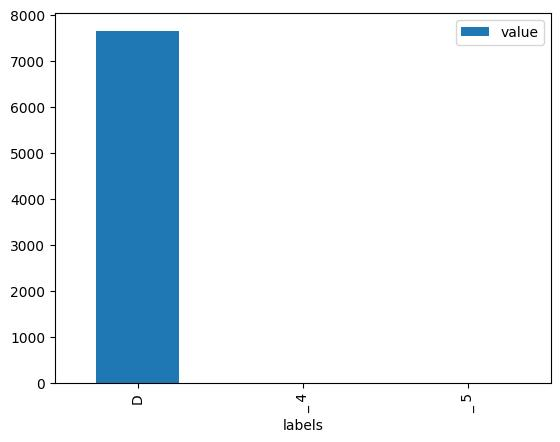
\includegraphics[width=1\textwidth]{assets/ca_1.jpg}
                        \end{figure}
                            \end{columns}
        
        Le point de vente avec le CA le plus élevé à \textbf{12 069€}, est \textbf{C}.\par
        Le point de vente \textbf{B} avec \textbf{3 632€} représente le plus petit CA du mois.\par
        La visualisation ci-dessus présente la somme des quantités commandées (PERMANENT + NON PERMANENT) par point de vente.\par
        \textbf{C} est le point de vente ayant commandé le plus d’UVC : \textbf{5 753 UVC au mois de ???}.\par
        Le point de vente \textbf{B} avec : \textbf{1 745 UVC} représente la plus faible quantité du mois.\par
    \end{frame}

    \subsection{Localisation}
    \subsection{Activité}

    \begin{frame}[plain]
        \tiny
        \frametitle{Localisation}

        \begin{columns}
            \column{0.66\textwidth}
                La visualisation ci-contre présente la répartition du CA du mois dernier par localisation :

                \begin{itemize}
                                            \item{Les points de vente \textbf{Continent} représentent \textbf{76.7\%} du CA}
                                            \item{Les points de vente \textbf{Corse} représentent \textbf{23.3\%} du CA}
                                    \end{itemize}

            \column{0.33\textwidth}
                \centering

                \begin{figure}[h]
                    \centering
                    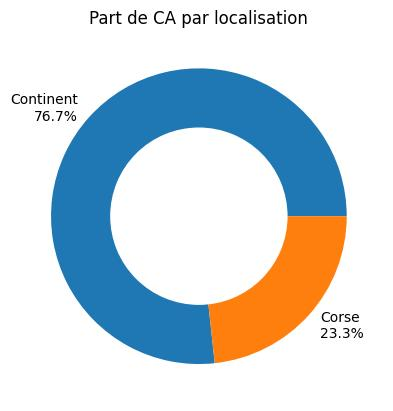
\includegraphics[width=1\textwidth]{assets/ca_par_localisation}
                \end{figure}
        \end{columns}

        {\hskip-3em\usebeamerfont{frametitle}\usebeamercolor[fg]{frametitle} Activité}

        \begin{columns}
            \column{0.33\textwidth}
                \centering

                \begin{figure}[h]
                    \centering
                    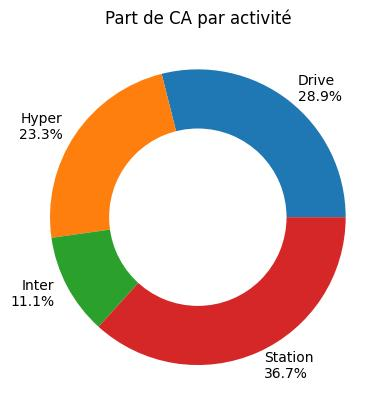
\includegraphics[width=1\textwidth]{assets/ca_par_activite}
                \end{figure}

            \column{0.66\textwidth}
                La visualisation ci-contre présente la répartition du CA par activité :

                \begin{itemize}
                                            \item{Les points de vente \textbf{Drive} représentent \textbf{28.9\%} du CA}
                                            \item{Les points de vente \textbf{Hyper} représentent \textbf{23.3\%} du CA}
                                            \item{Les points de vente \textbf{Inter} représentent \textbf{11.1\%} du CA}
                                            \item{Les points de vente \textbf{Station} représentent \textbf{36.7\%} du CA}
                                    \end{itemize}
        \end{columns}
    \end{frame}

    \section{Analyse du mode de gestion}
    \subsection{Non permanent}

    \begin{frame}
    \end{frame}

    \subsection{Permanent}

    \begin{frame}
    \end{frame}

    \section{Analyse par article}
    \subsection{Articles les plus commandés}

    \begin{frame}
    \end{frame}

    \subsection{Articles les moins commandés}

    \begin{frame}
    \end{frame}

\end{document}
